\subsection{Performance}

\begin{figure*}
  \centering
  \begin{subfigure}[b]{\textwidth}
          \centering
          
\includegraphics[width=0.4\textwidth]{data/legend.pdf}
  \end{subfigure}

  \begin{subfigure}[b]{0.33\textwidth}
      \centering
      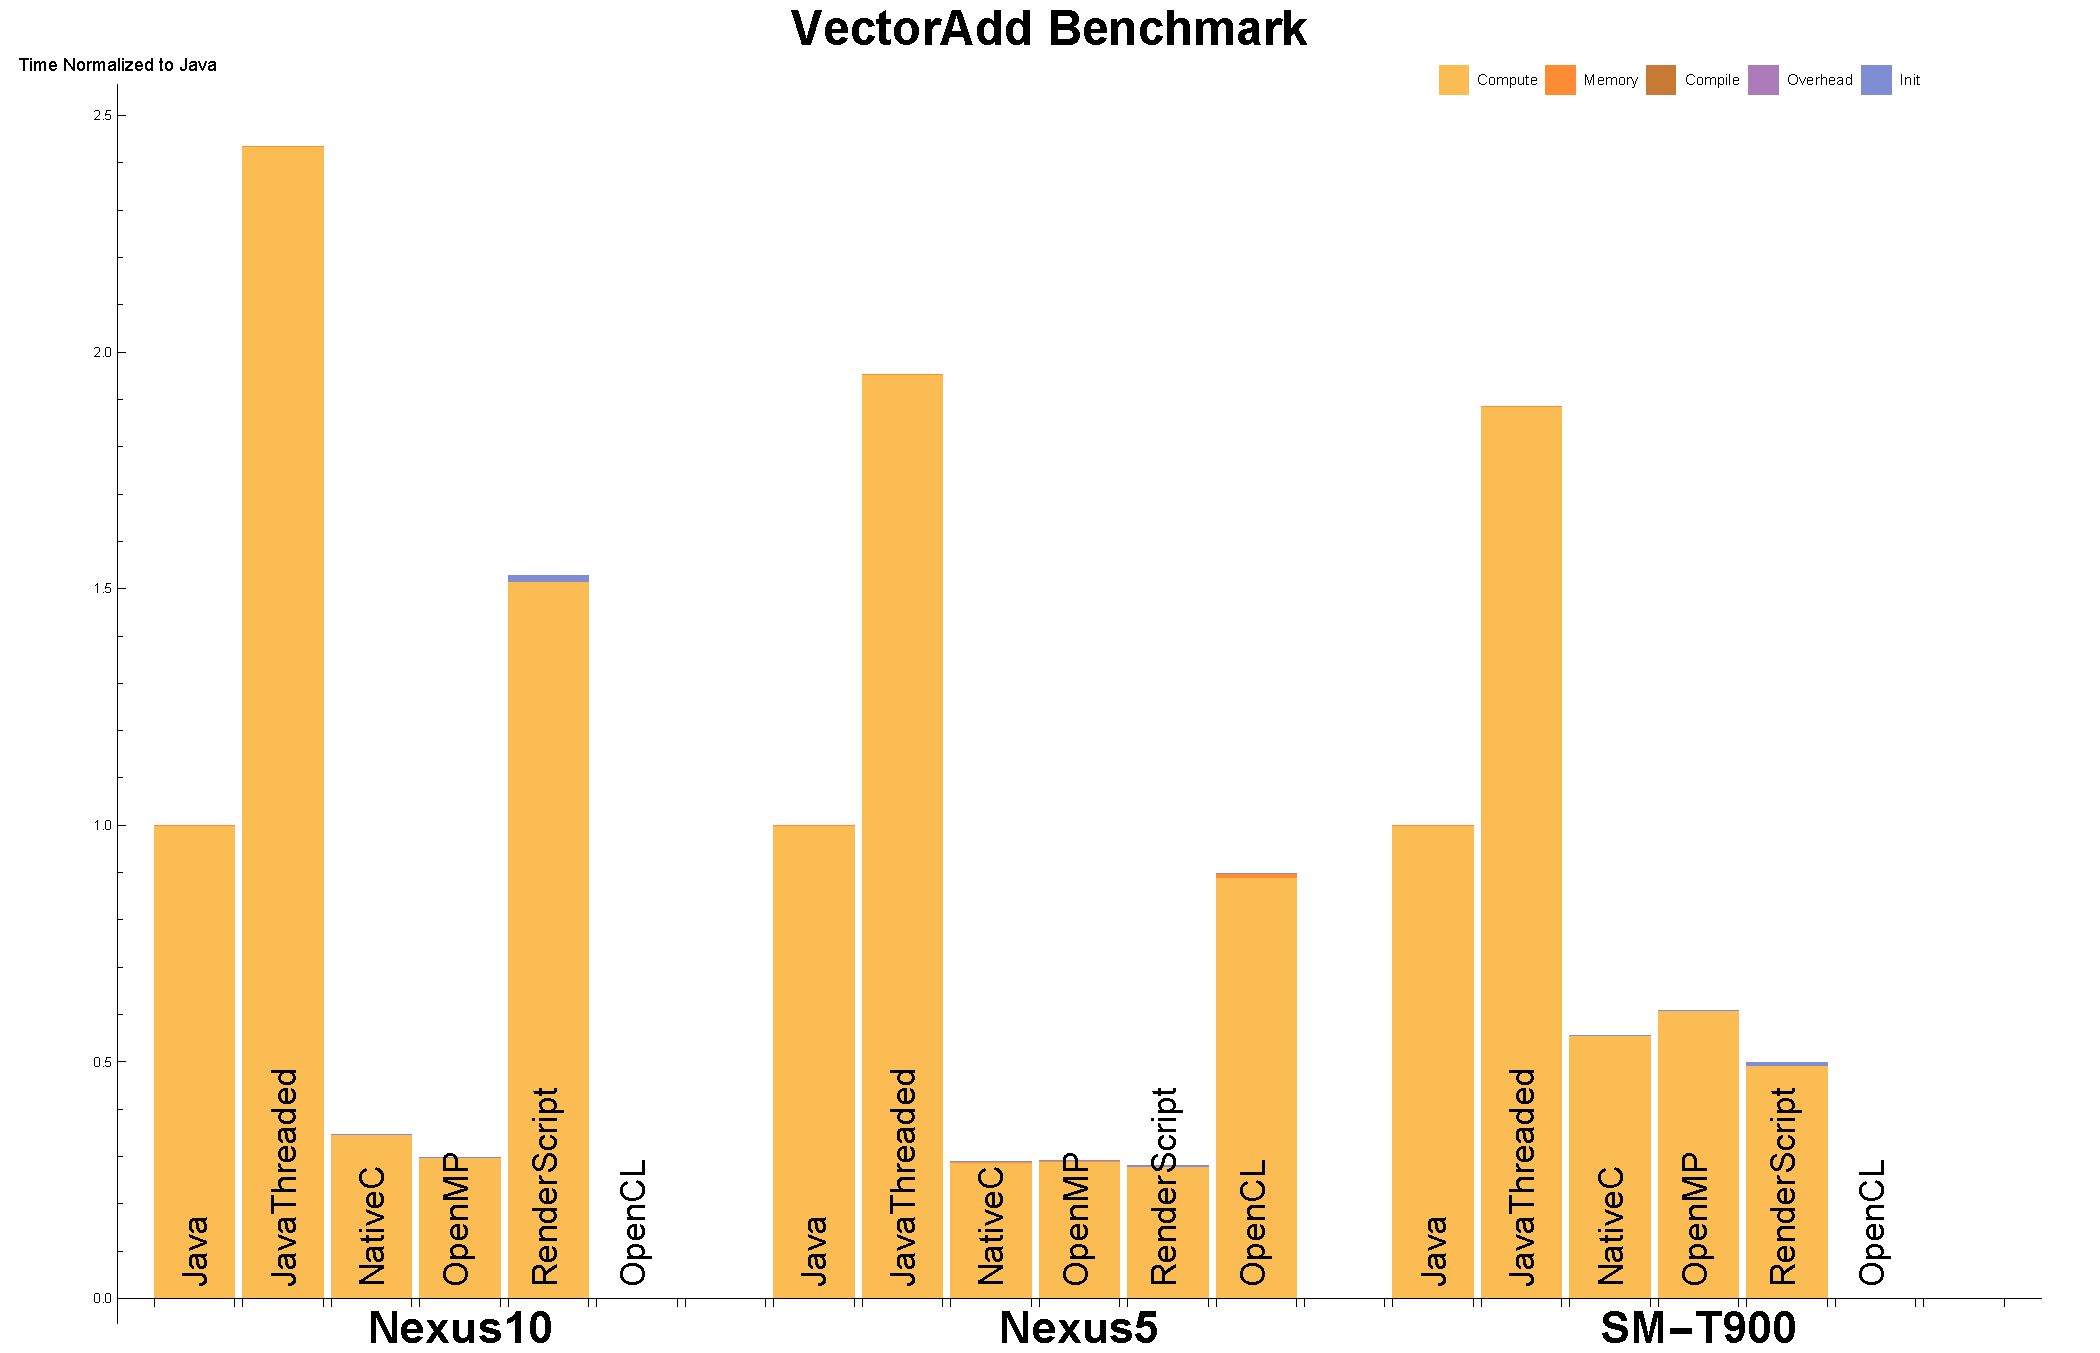
\includegraphics[width=0.9\textwidth]{data/VectorAdd_onecompute_time.pdf}
      \caption{VectorAdd}
  \end{subfigure}
  \begin{subfigure}[b]{0.33\textwidth}
      \centering
      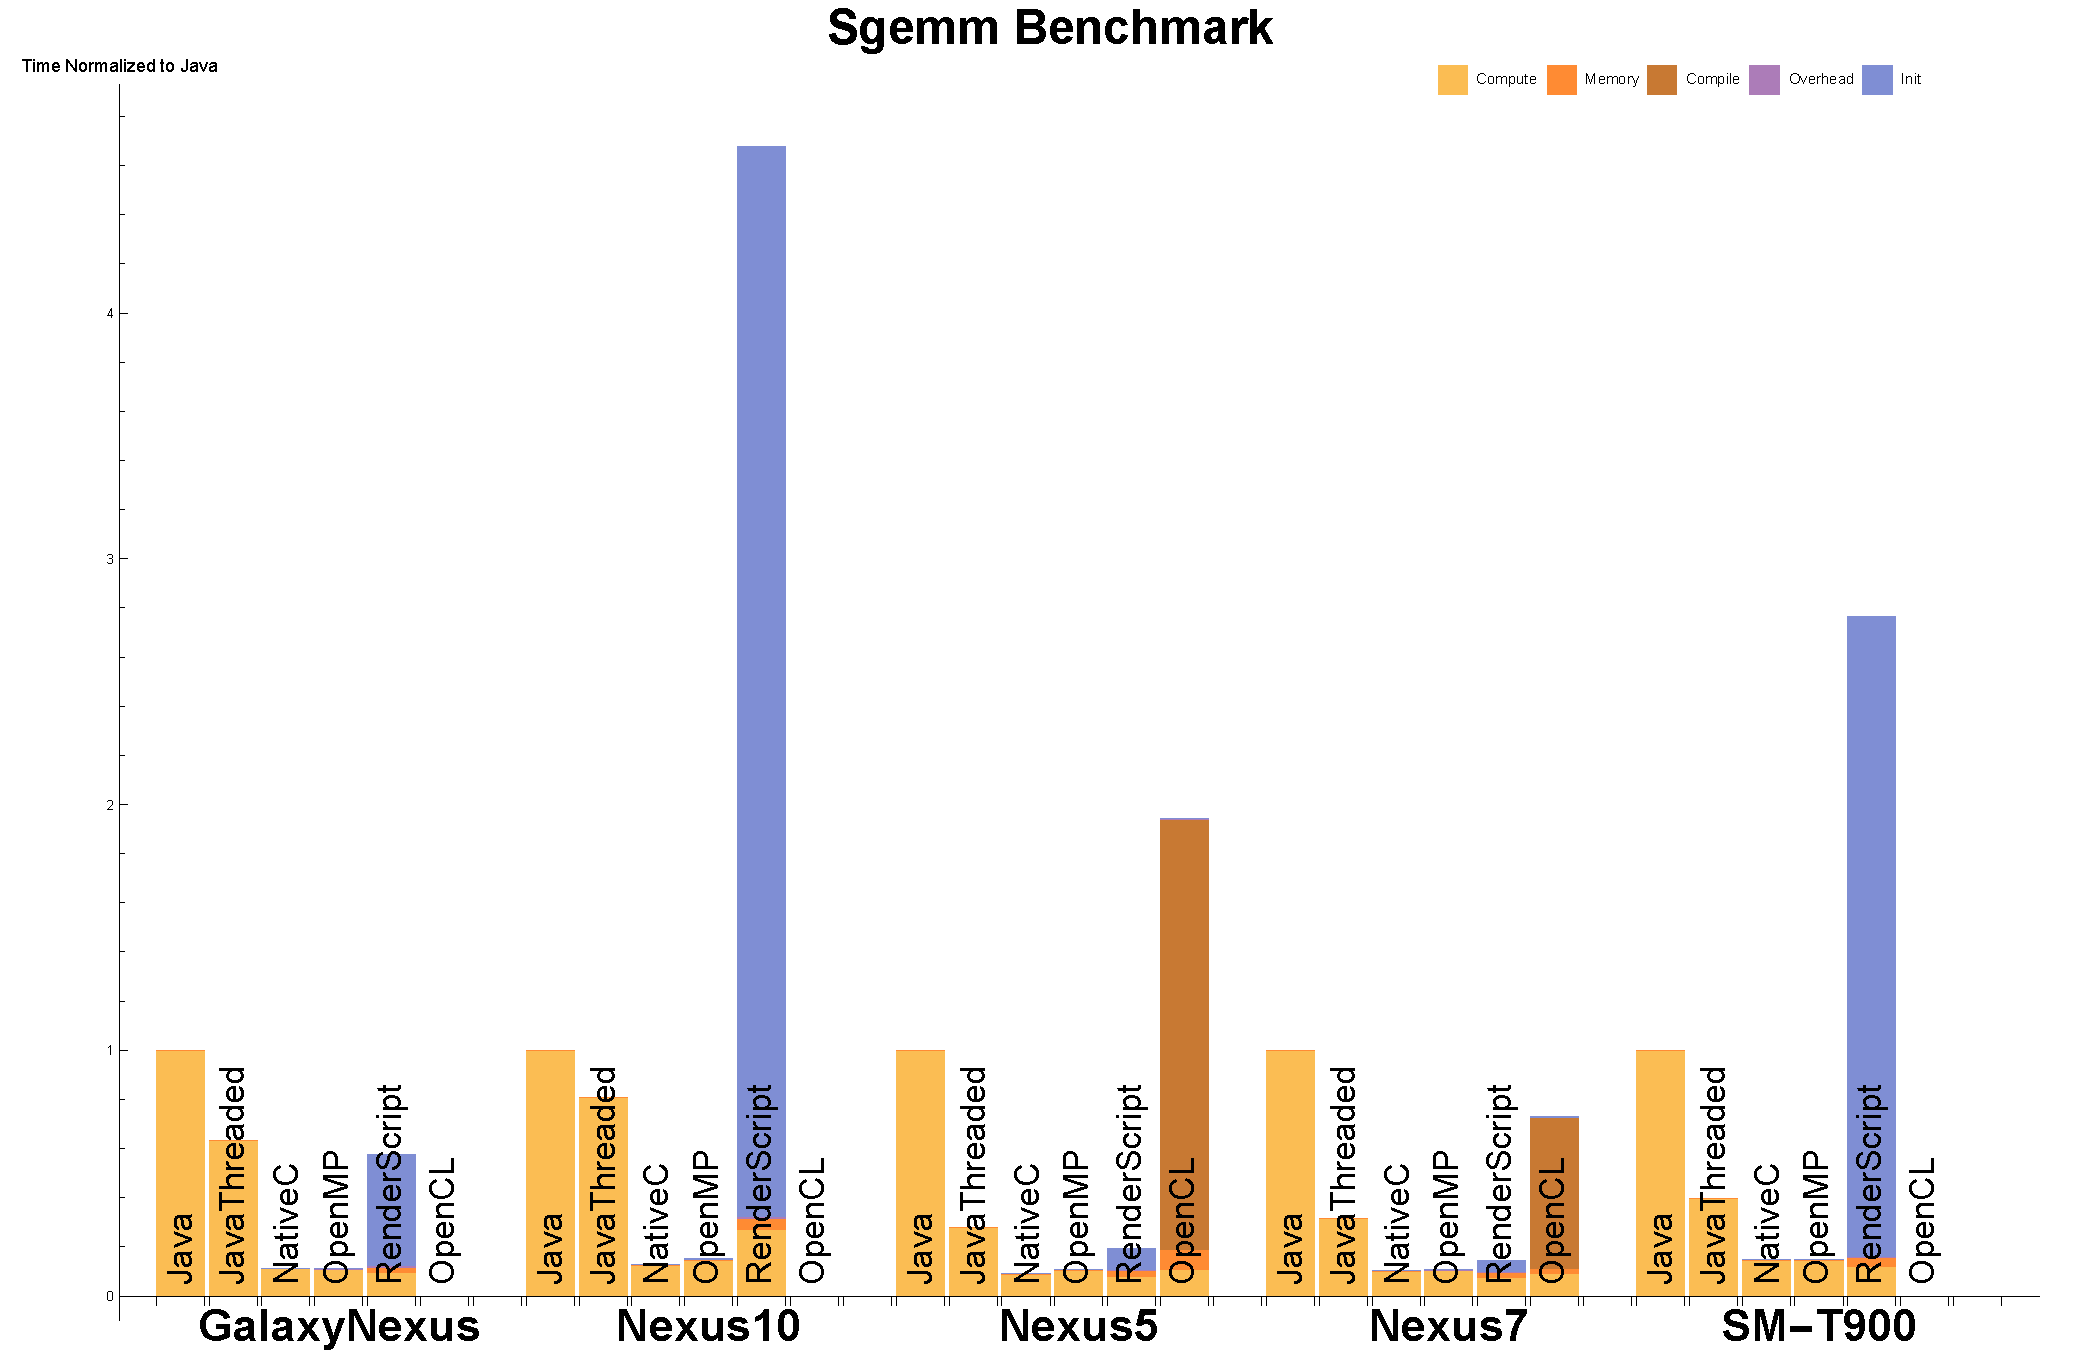
\includegraphics[width=0.9\textwidth]{data/Sgemm_onecompute_time.pdf}
      \caption{Sgemm}
  \end{subfigure}
  \begin{subfigure}[b]{0.33\textwidth}
      \centering
      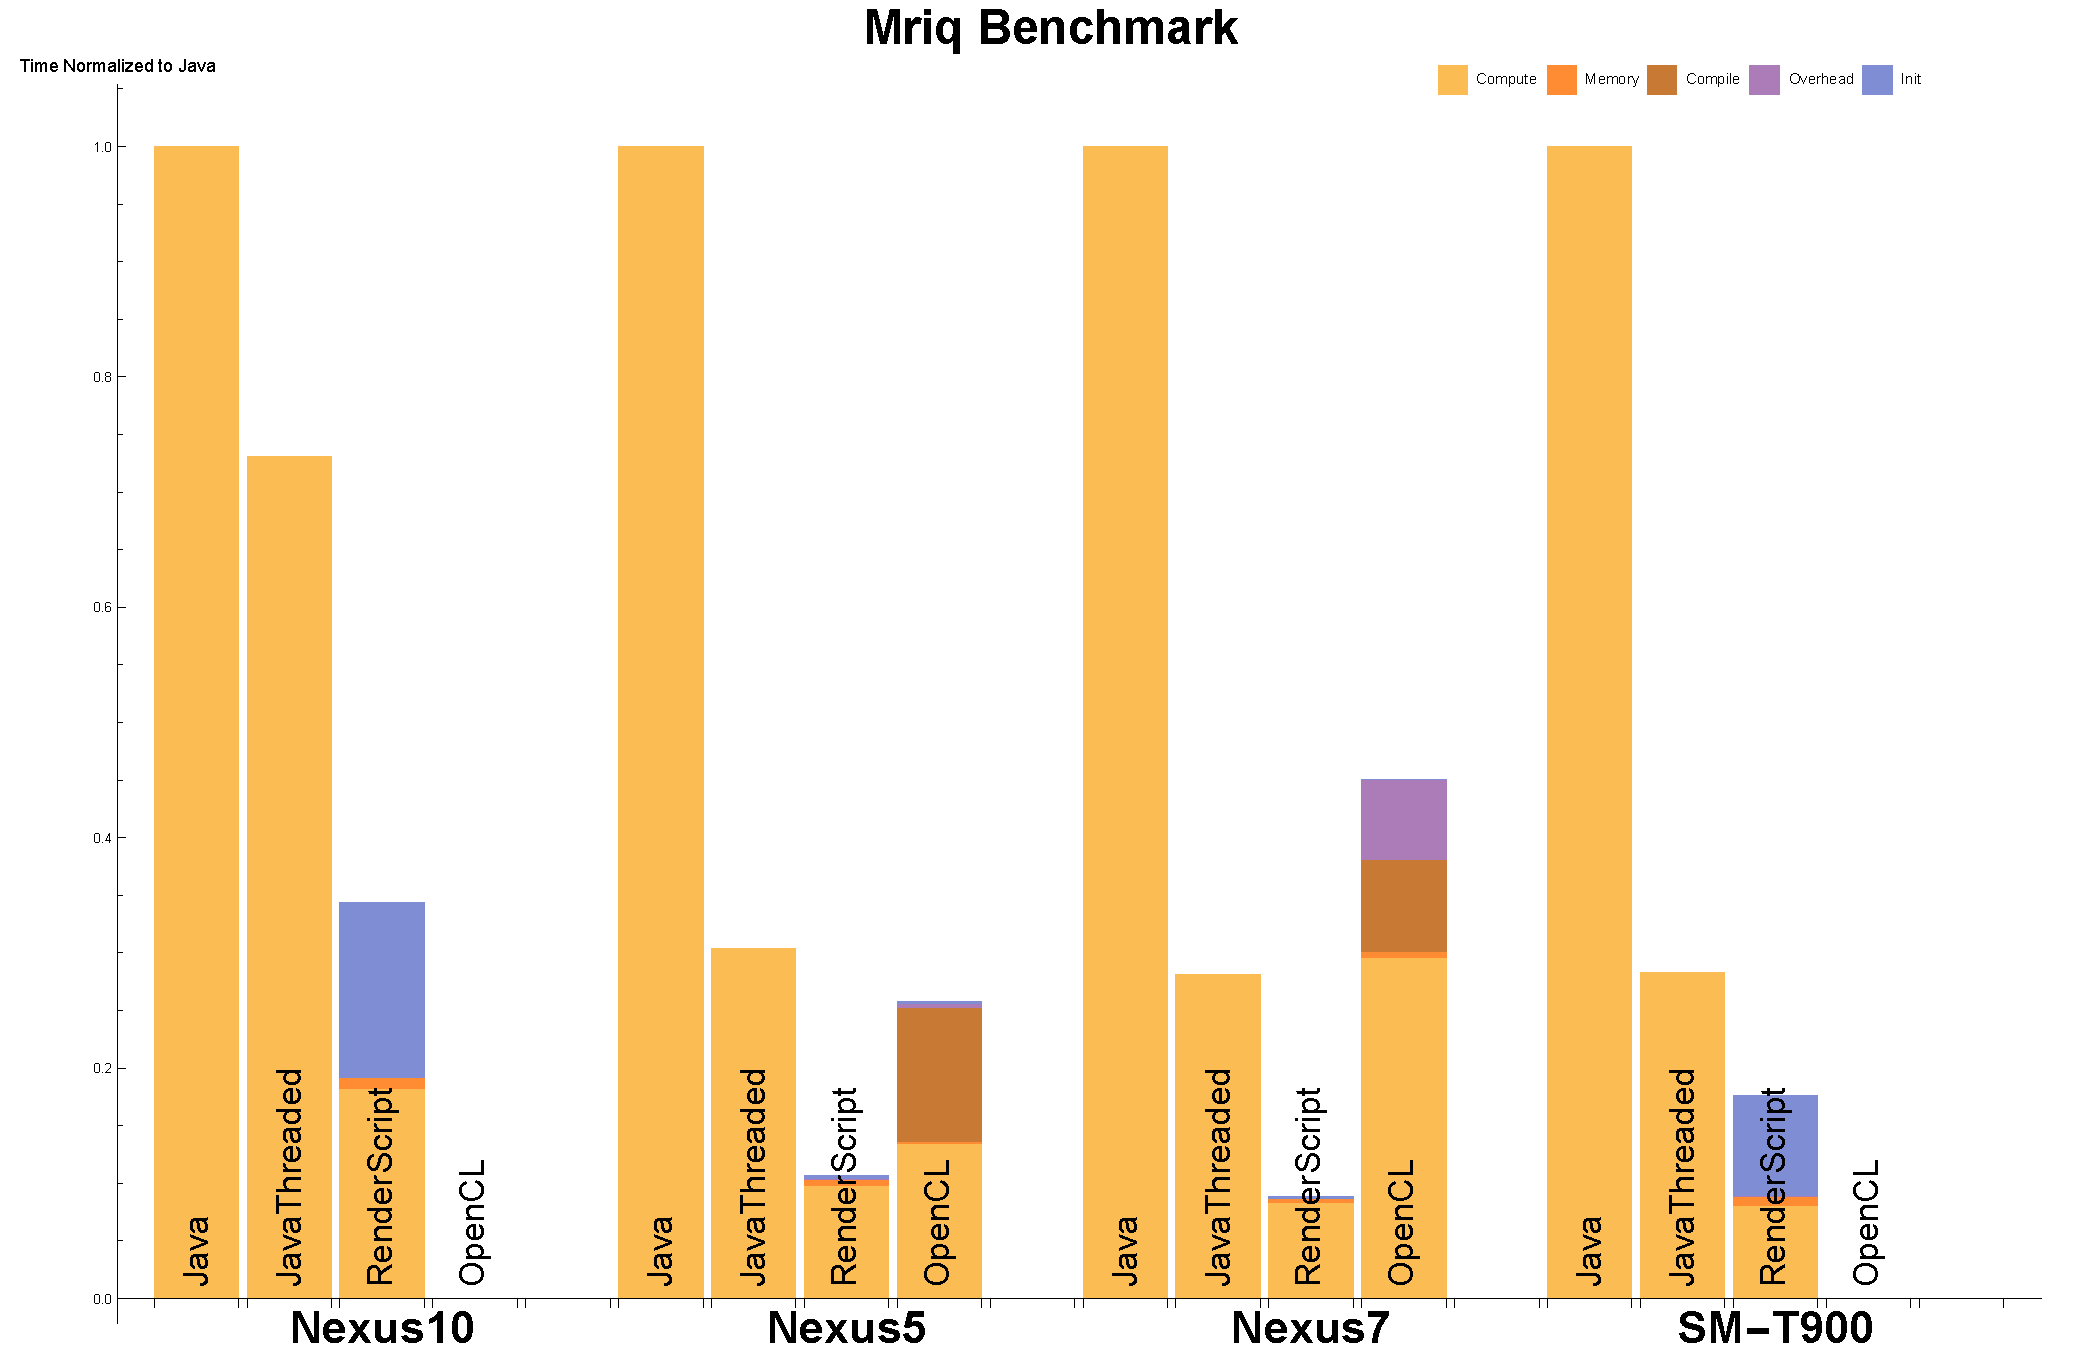
\includegraphics[width=0.9\textwidth]{data/Mriq_onecompute_time.pdf}
      \caption{MRIQ}
  \end{subfigure}

  \begin{subfigure}[b]{0.33\textwidth}
      \centering
      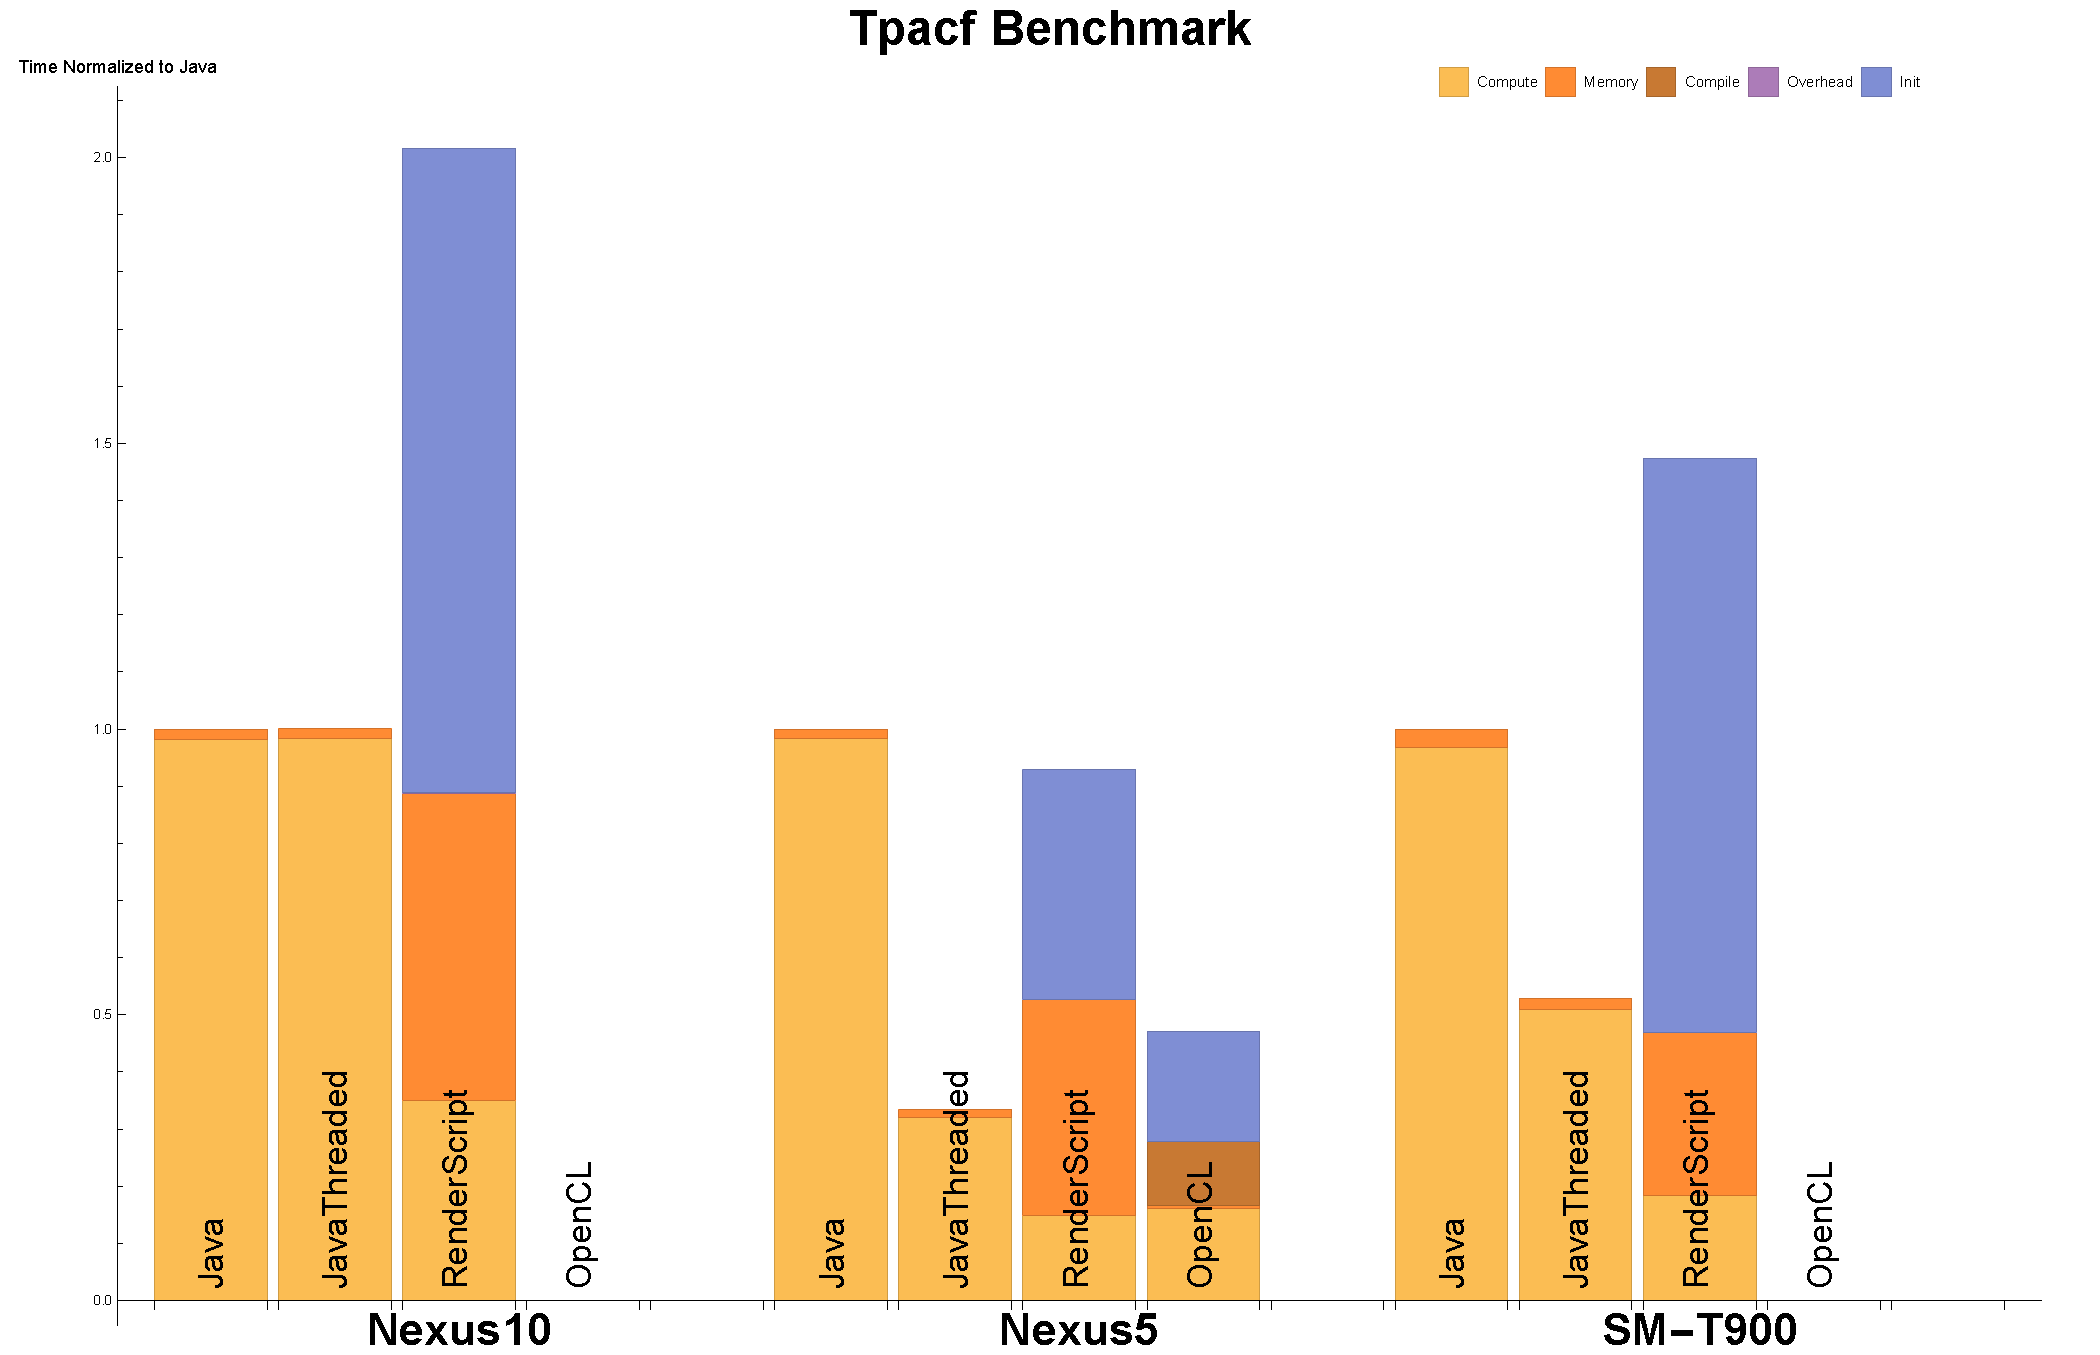
\includegraphics[width=0.9\textwidth]{data/Tpacf_onecompute_time.pdf}
      \caption{TPACF}
  \end{subfigure}
  \begin{subfigure}[b]{0.33\textwidth}
      \centering
      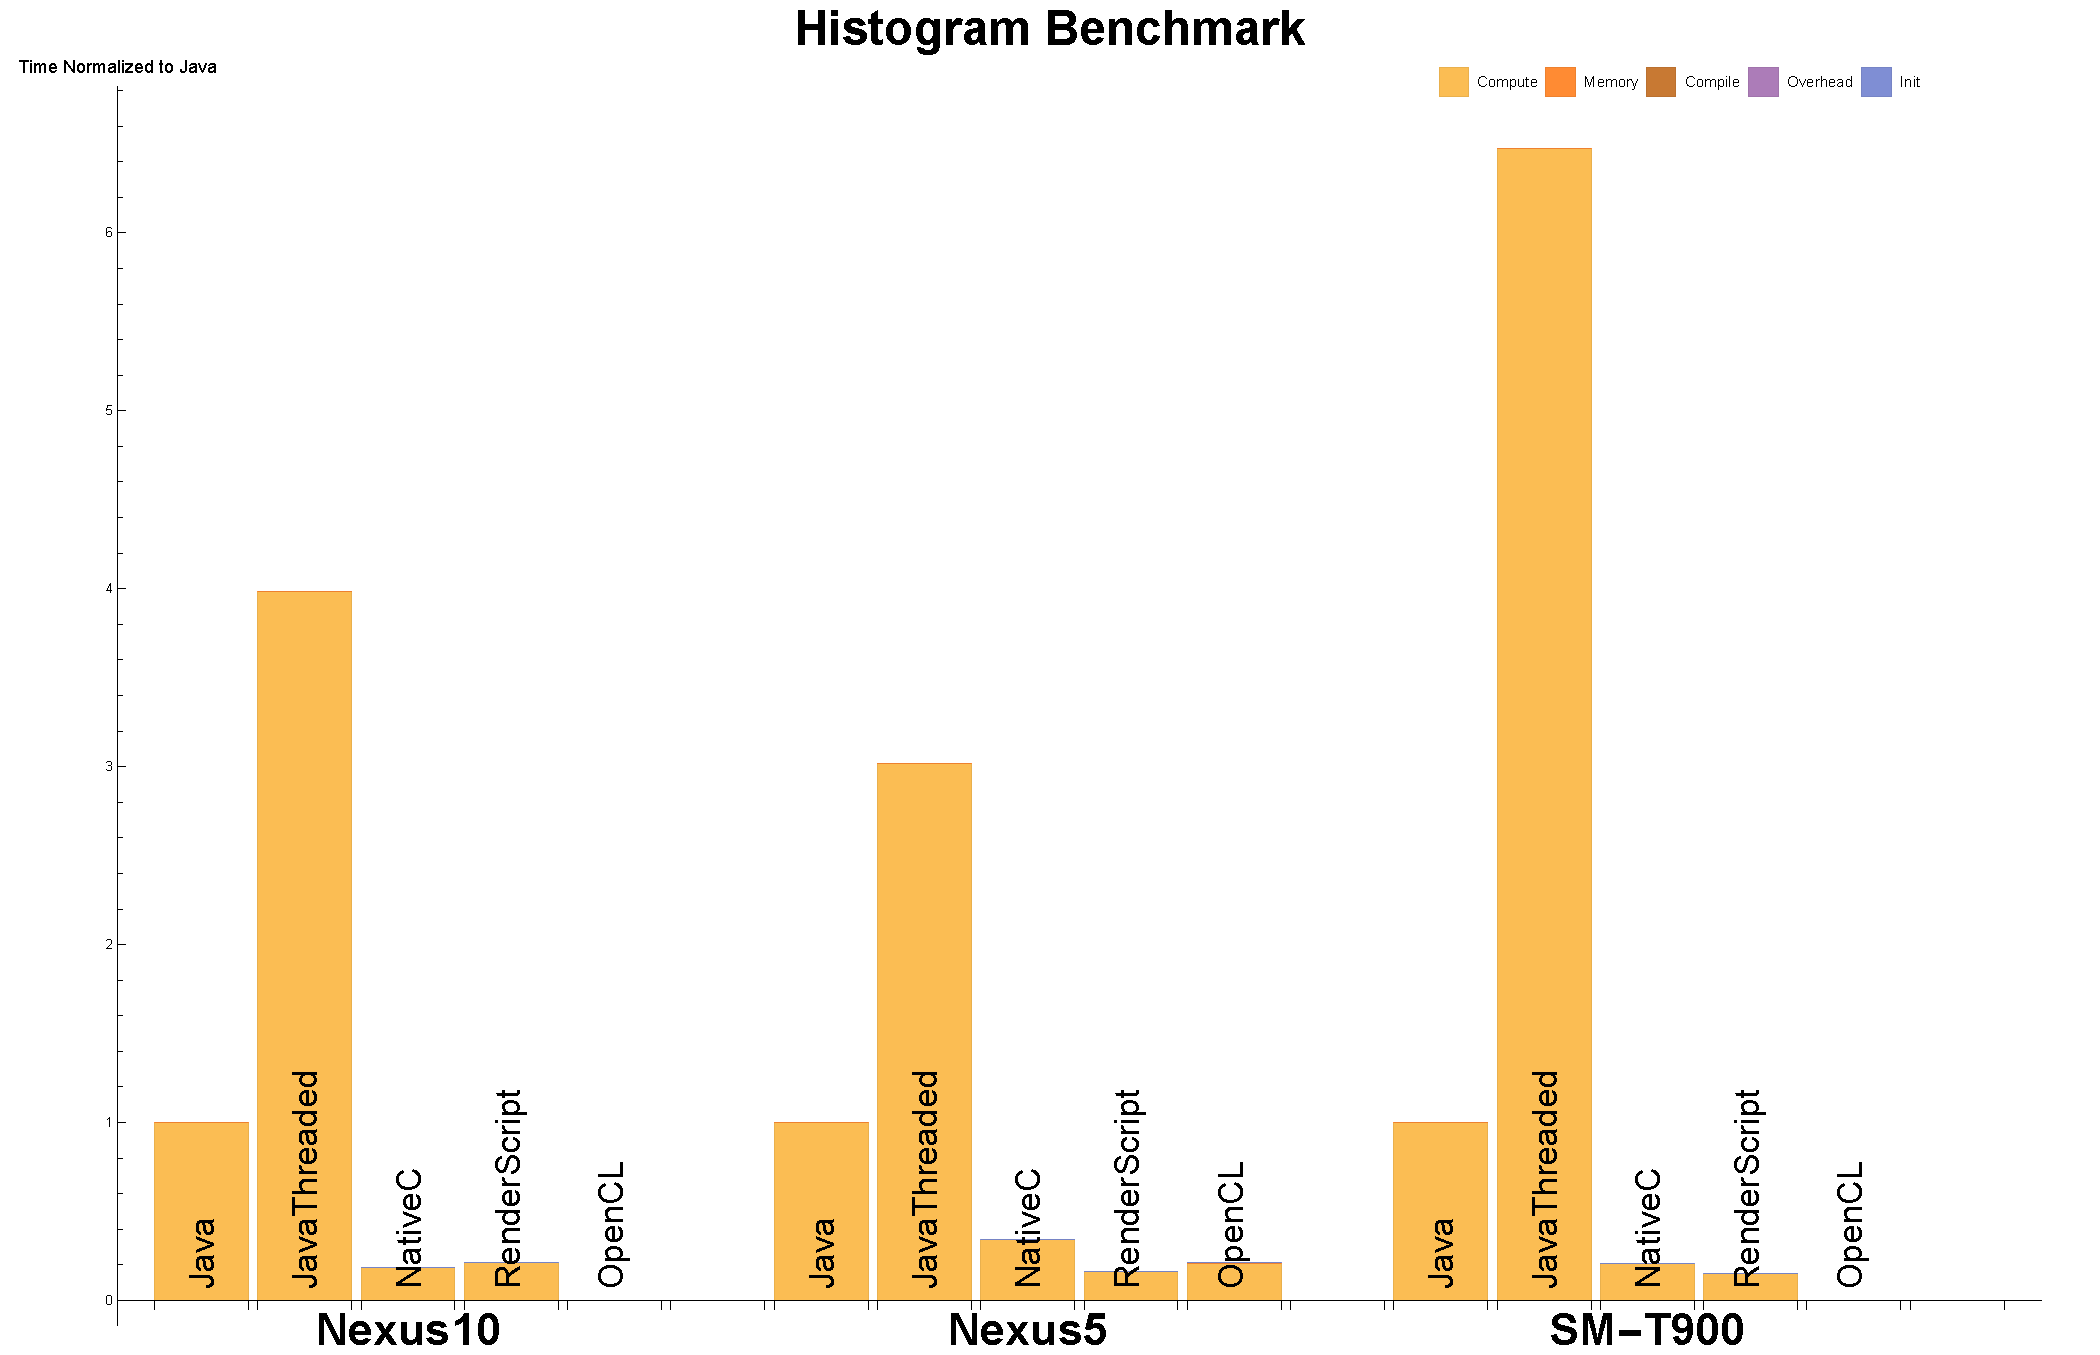
\includegraphics[width=0.9\textwidth]{data/Histogram_onecompute_time.pdf}
      \caption{Histogram}
  \end{subfigure}
  \begin{subfigure}[b]{0.33\textwidth}
      \centering
      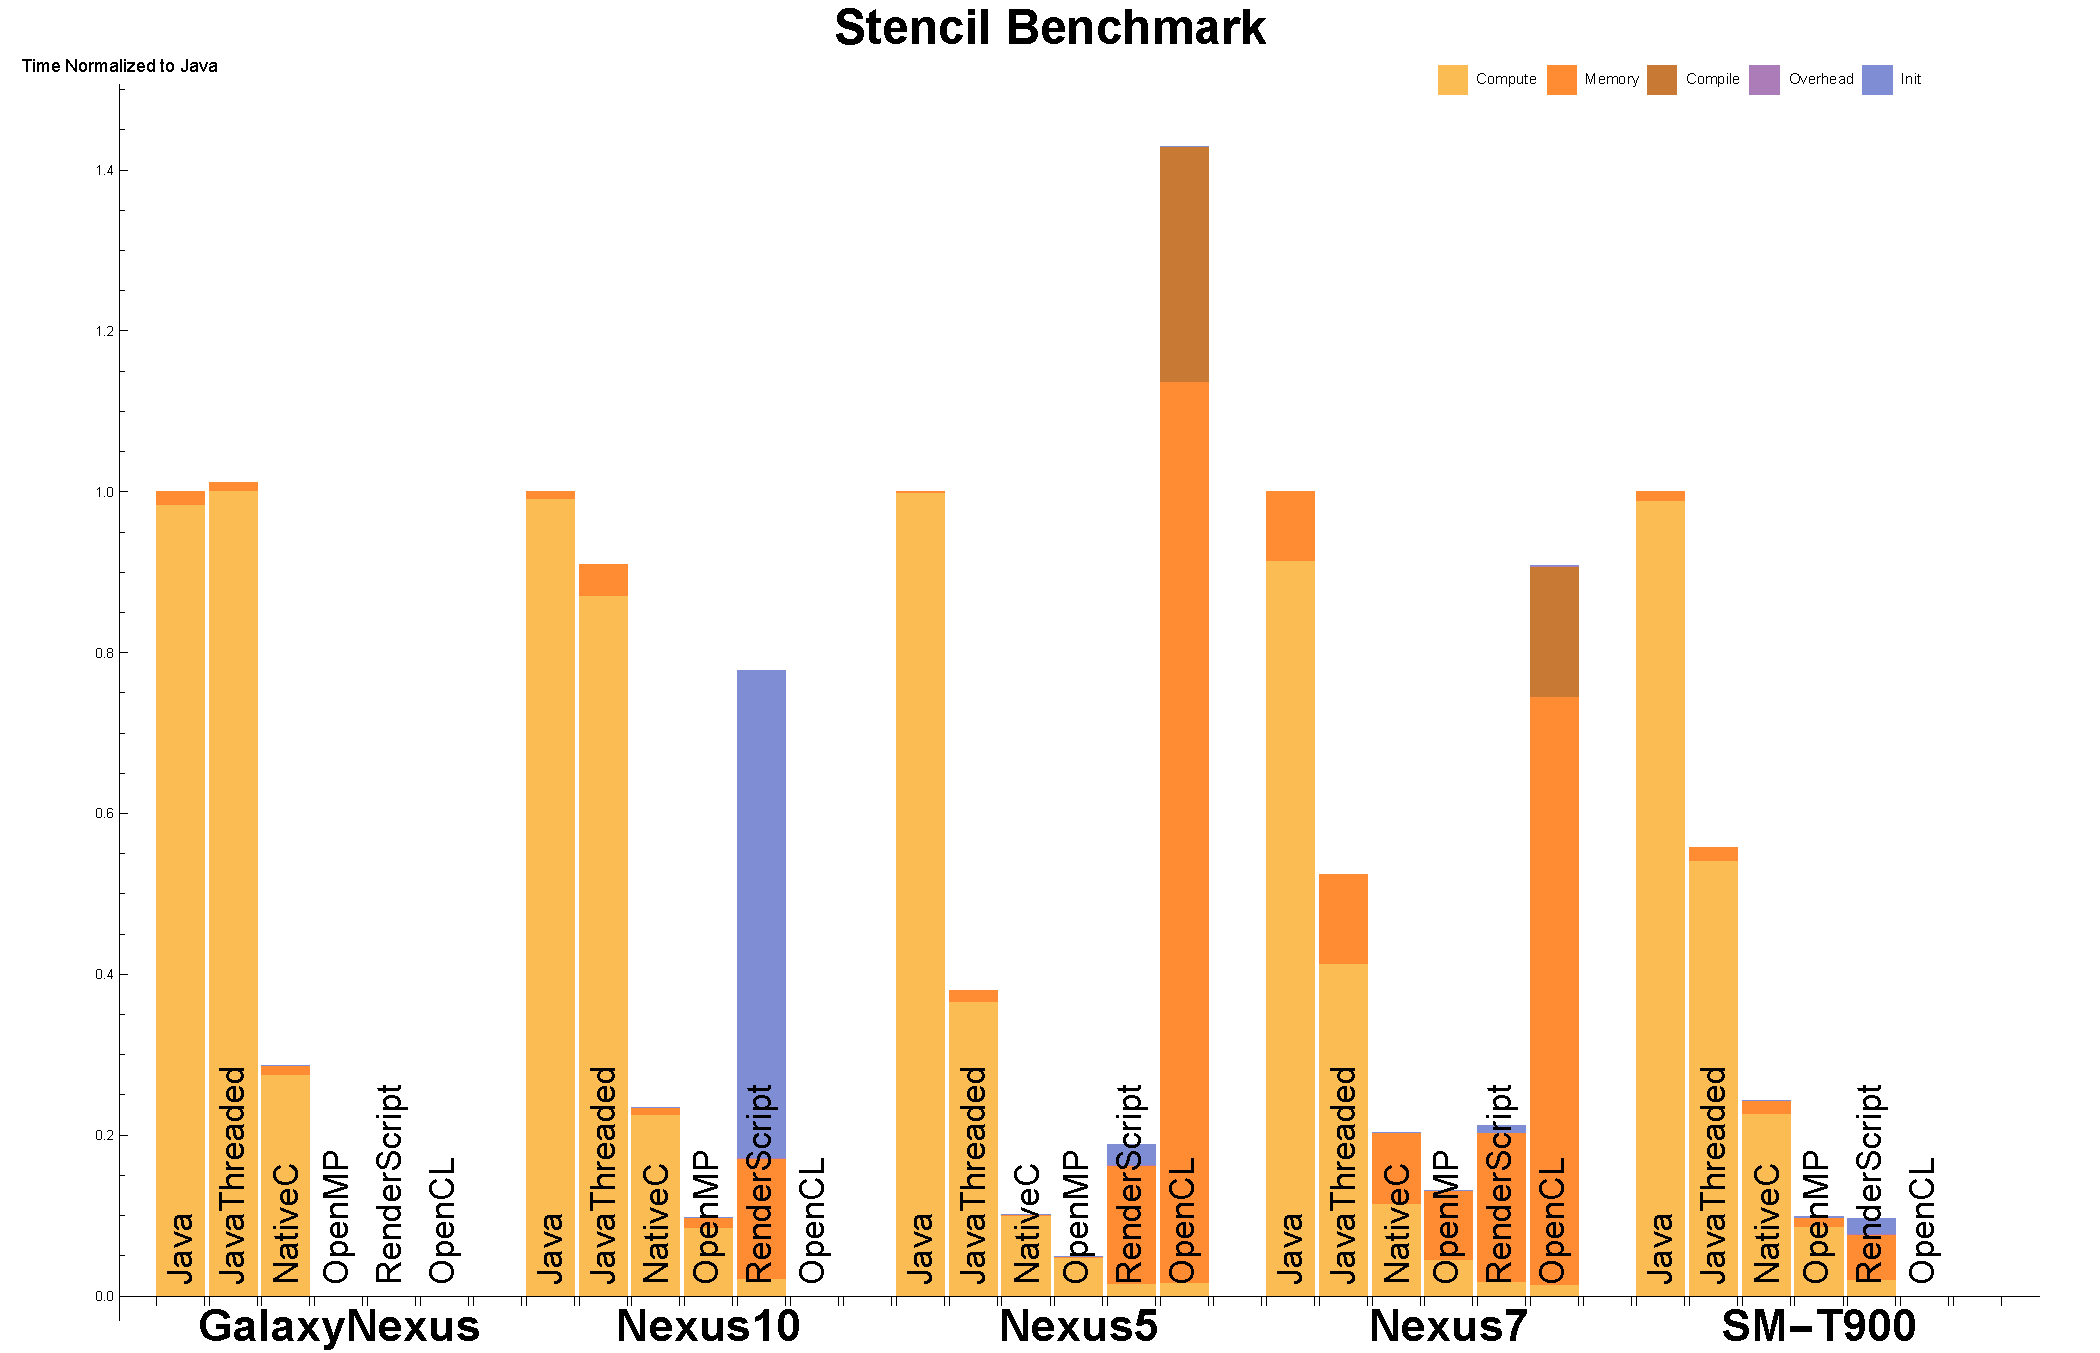
\includegraphics[width=0.9\textwidth]{data/Stencil_onecompute_time.pdf}
      \caption{Stencil}
  \end{subfigure}
  \caption{Runtime across devices where kernel is executed once. The runtimes are normalized to the Java execution time (lower is better). J : Java, JT : JavaThreaded, C : Native C, OMP: OpenMP, OCL : OpenCL, and RS : Renderscript.}
  \label{fig:perfOne}
\end{figure*}

\begin{figure*}

  \centering
  \begin{subfigure}[b]{\textwidth}
          \centering
          
\includegraphics[width=0.4\textwidth]{data/legend.pdf}
  \end{subfigure}

  \begin{subfigure}[b]{0.33\textwidth}
      \centering
      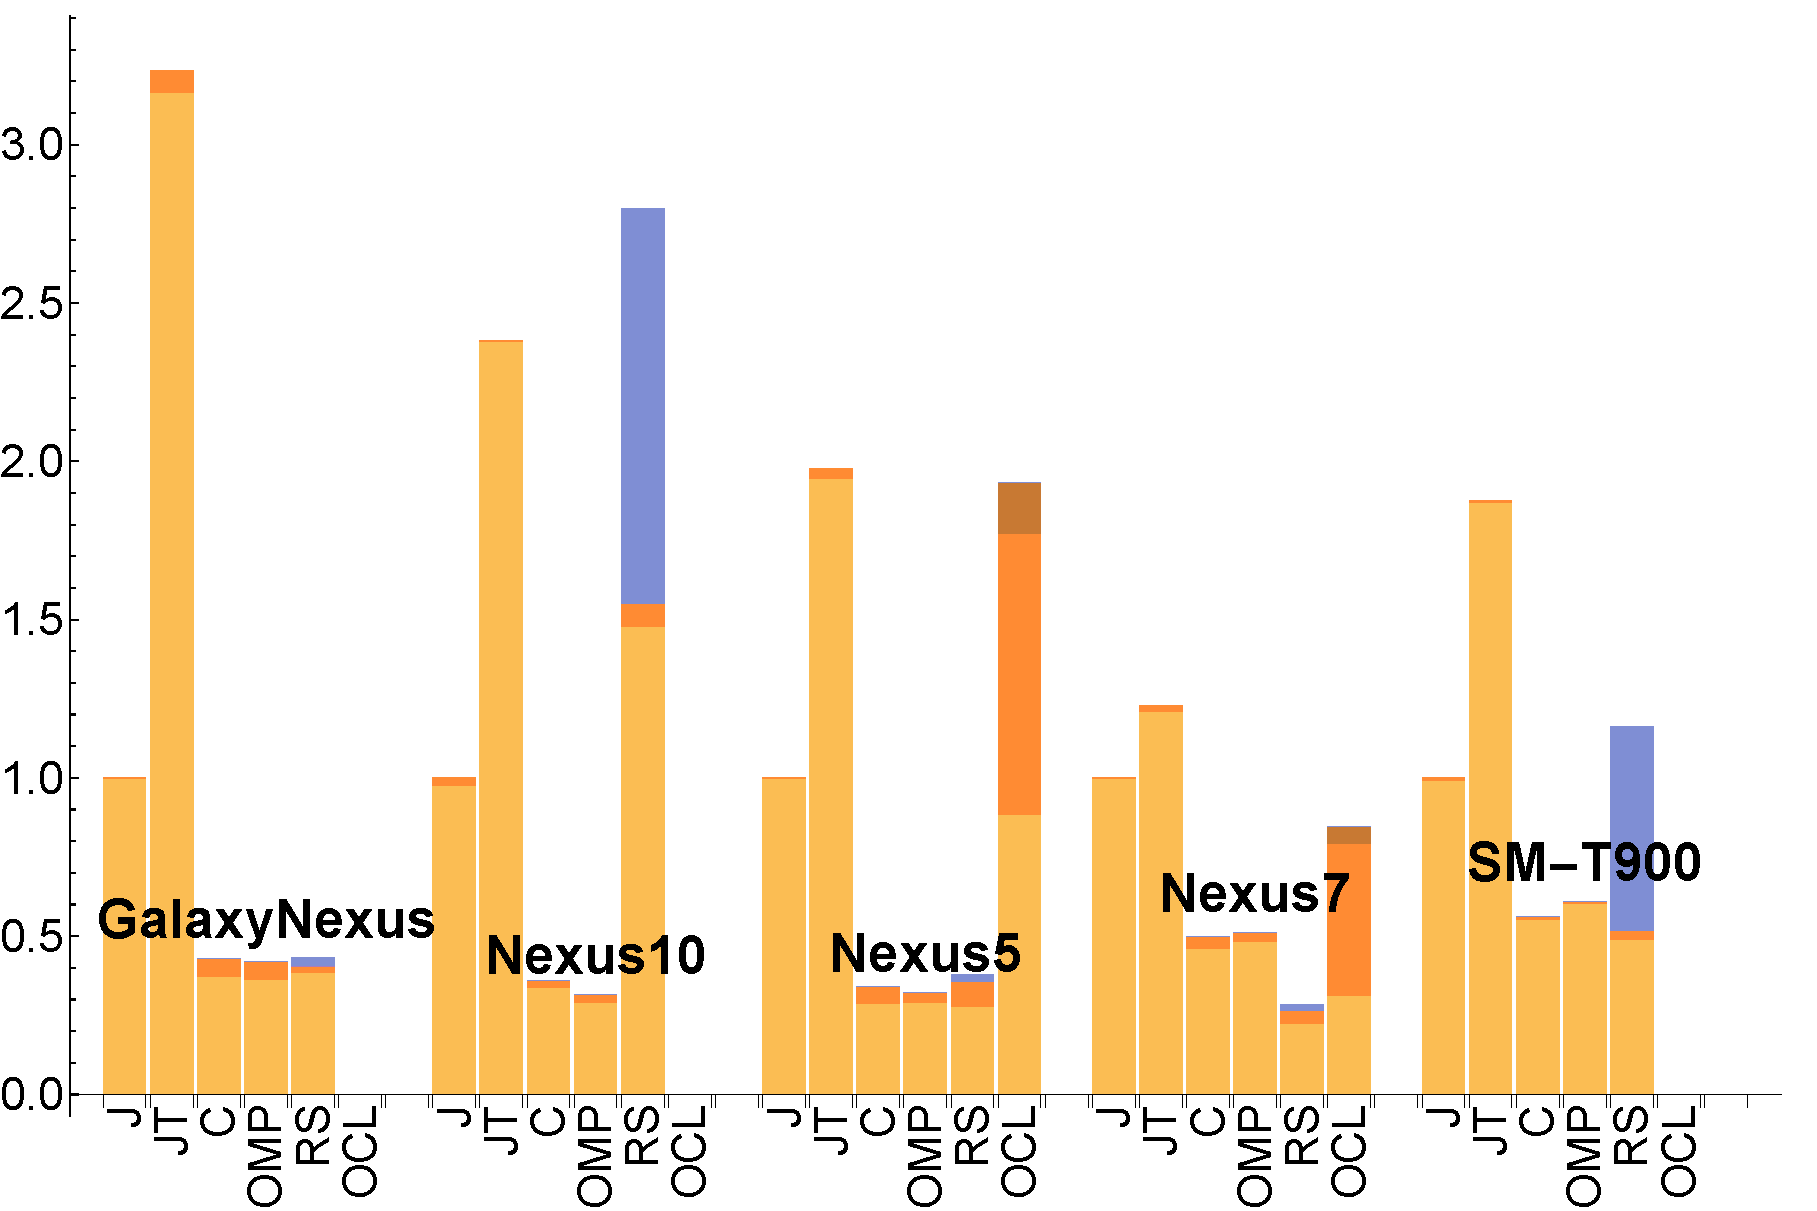
\includegraphics[width=0.9\textwidth]{data/VectorAdd_time.pdf}
      \caption{VectorAdd}
  \end{subfigure}
  \begin{subfigure}[b]{0.33\textwidth}
      \centering
      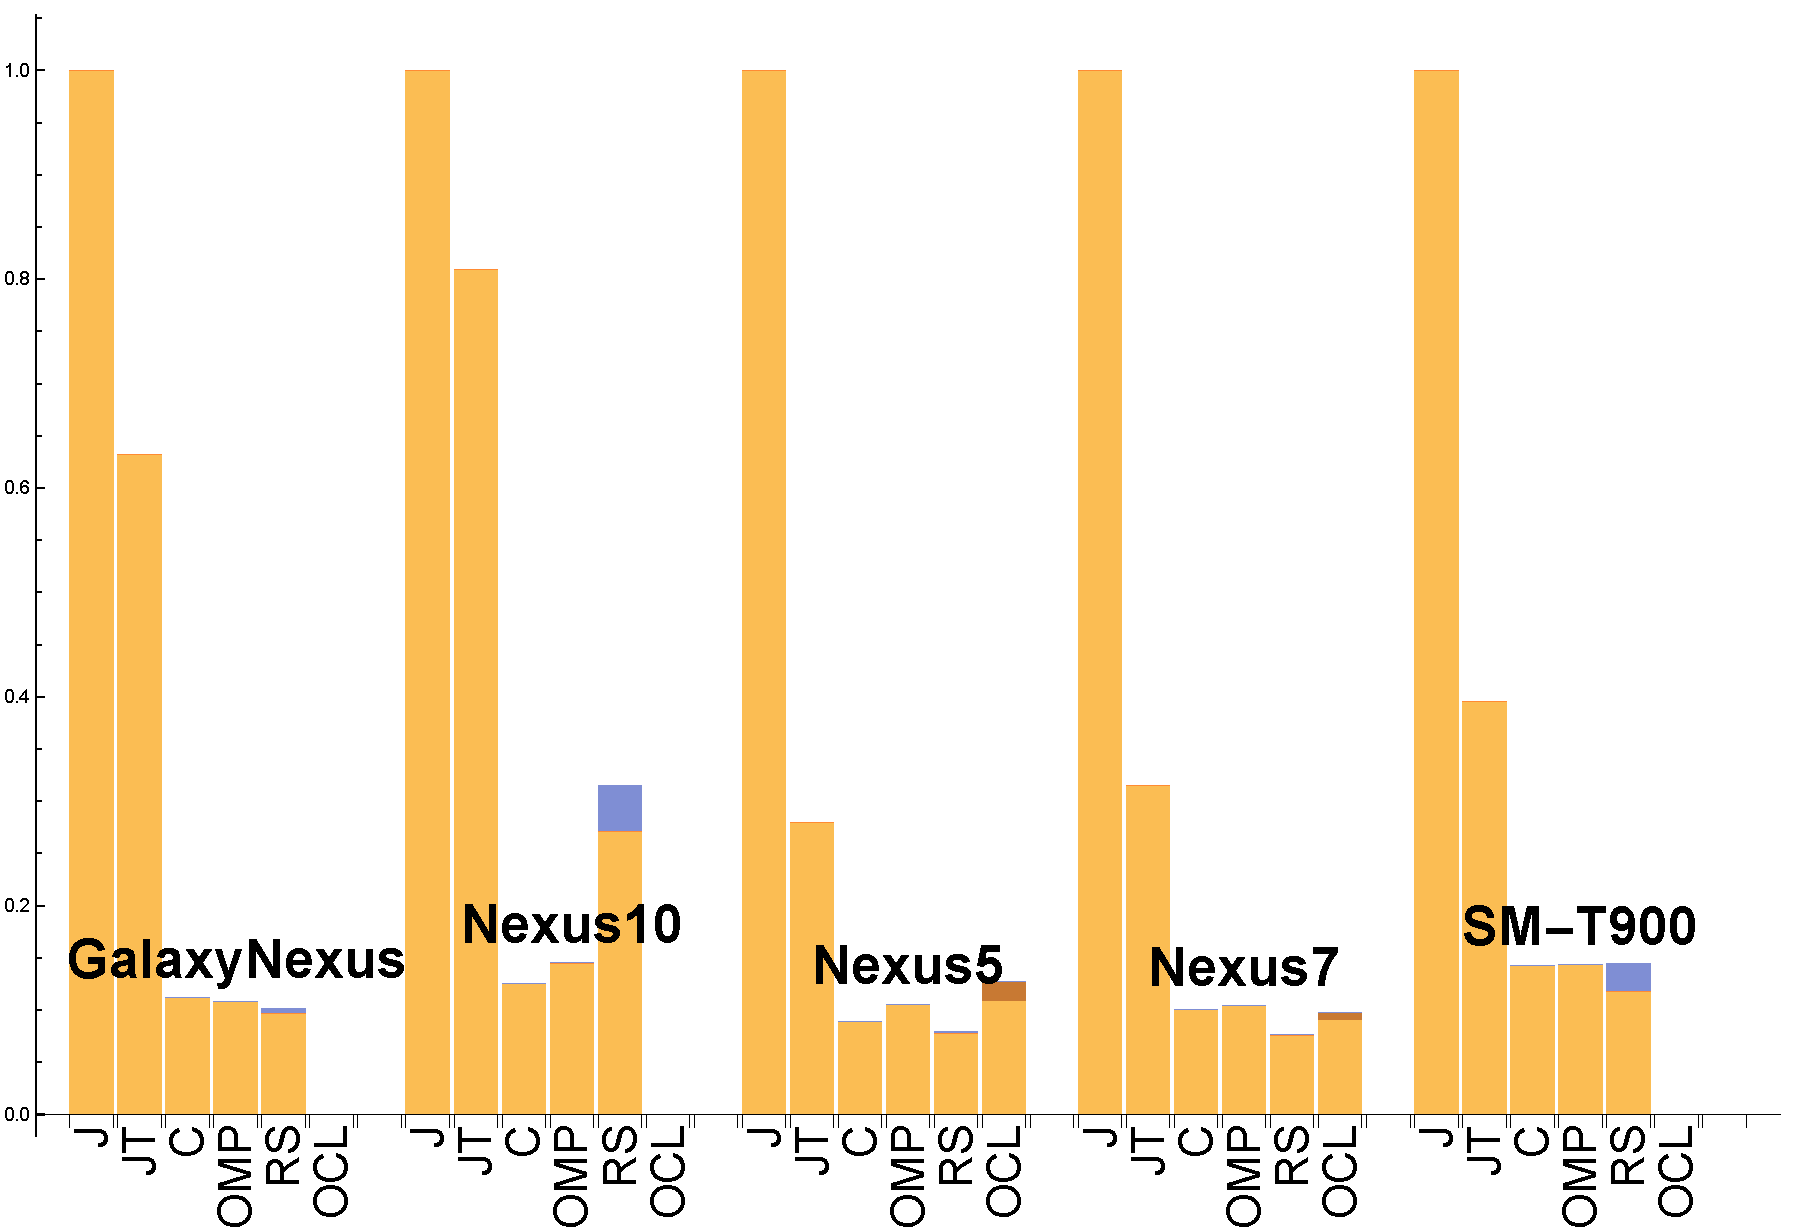
\includegraphics[width=0.9\textwidth]{data/Sgemm_time.pdf}
      \caption{Sgemm}
  \end{subfigure}
  \begin{subfigure}[b]{0.33\textwidth}
      \centering
      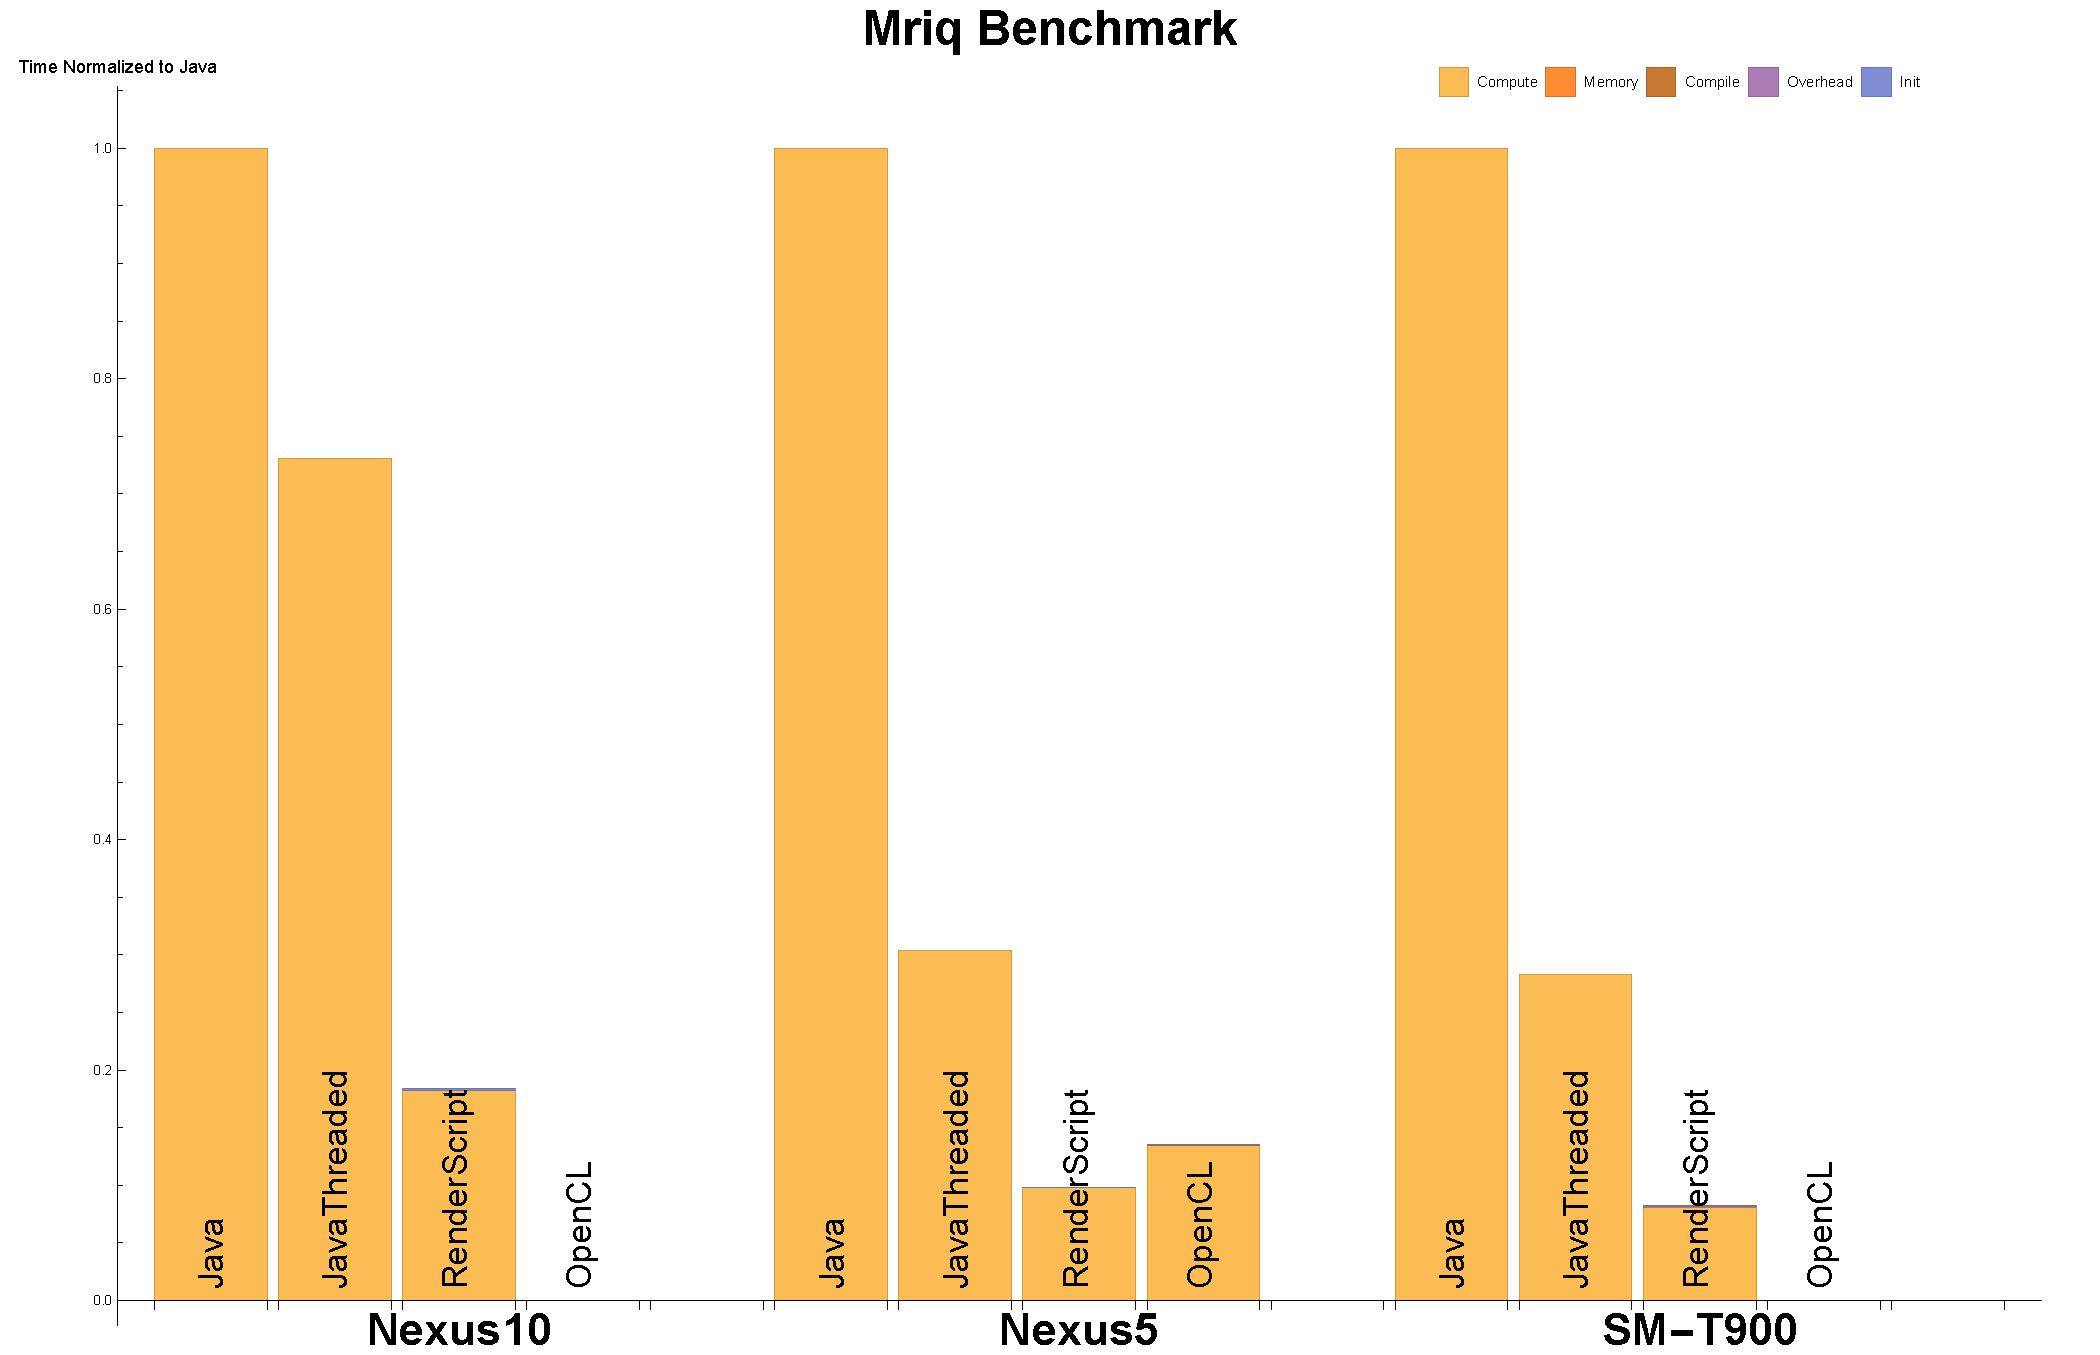
\includegraphics[width=0.9\textwidth]{data/Mriq_time.pdf}
      \caption{MRIQ}
  \end{subfigure}

  \begin{subfigure}[b]{0.33\textwidth}
      \centering
      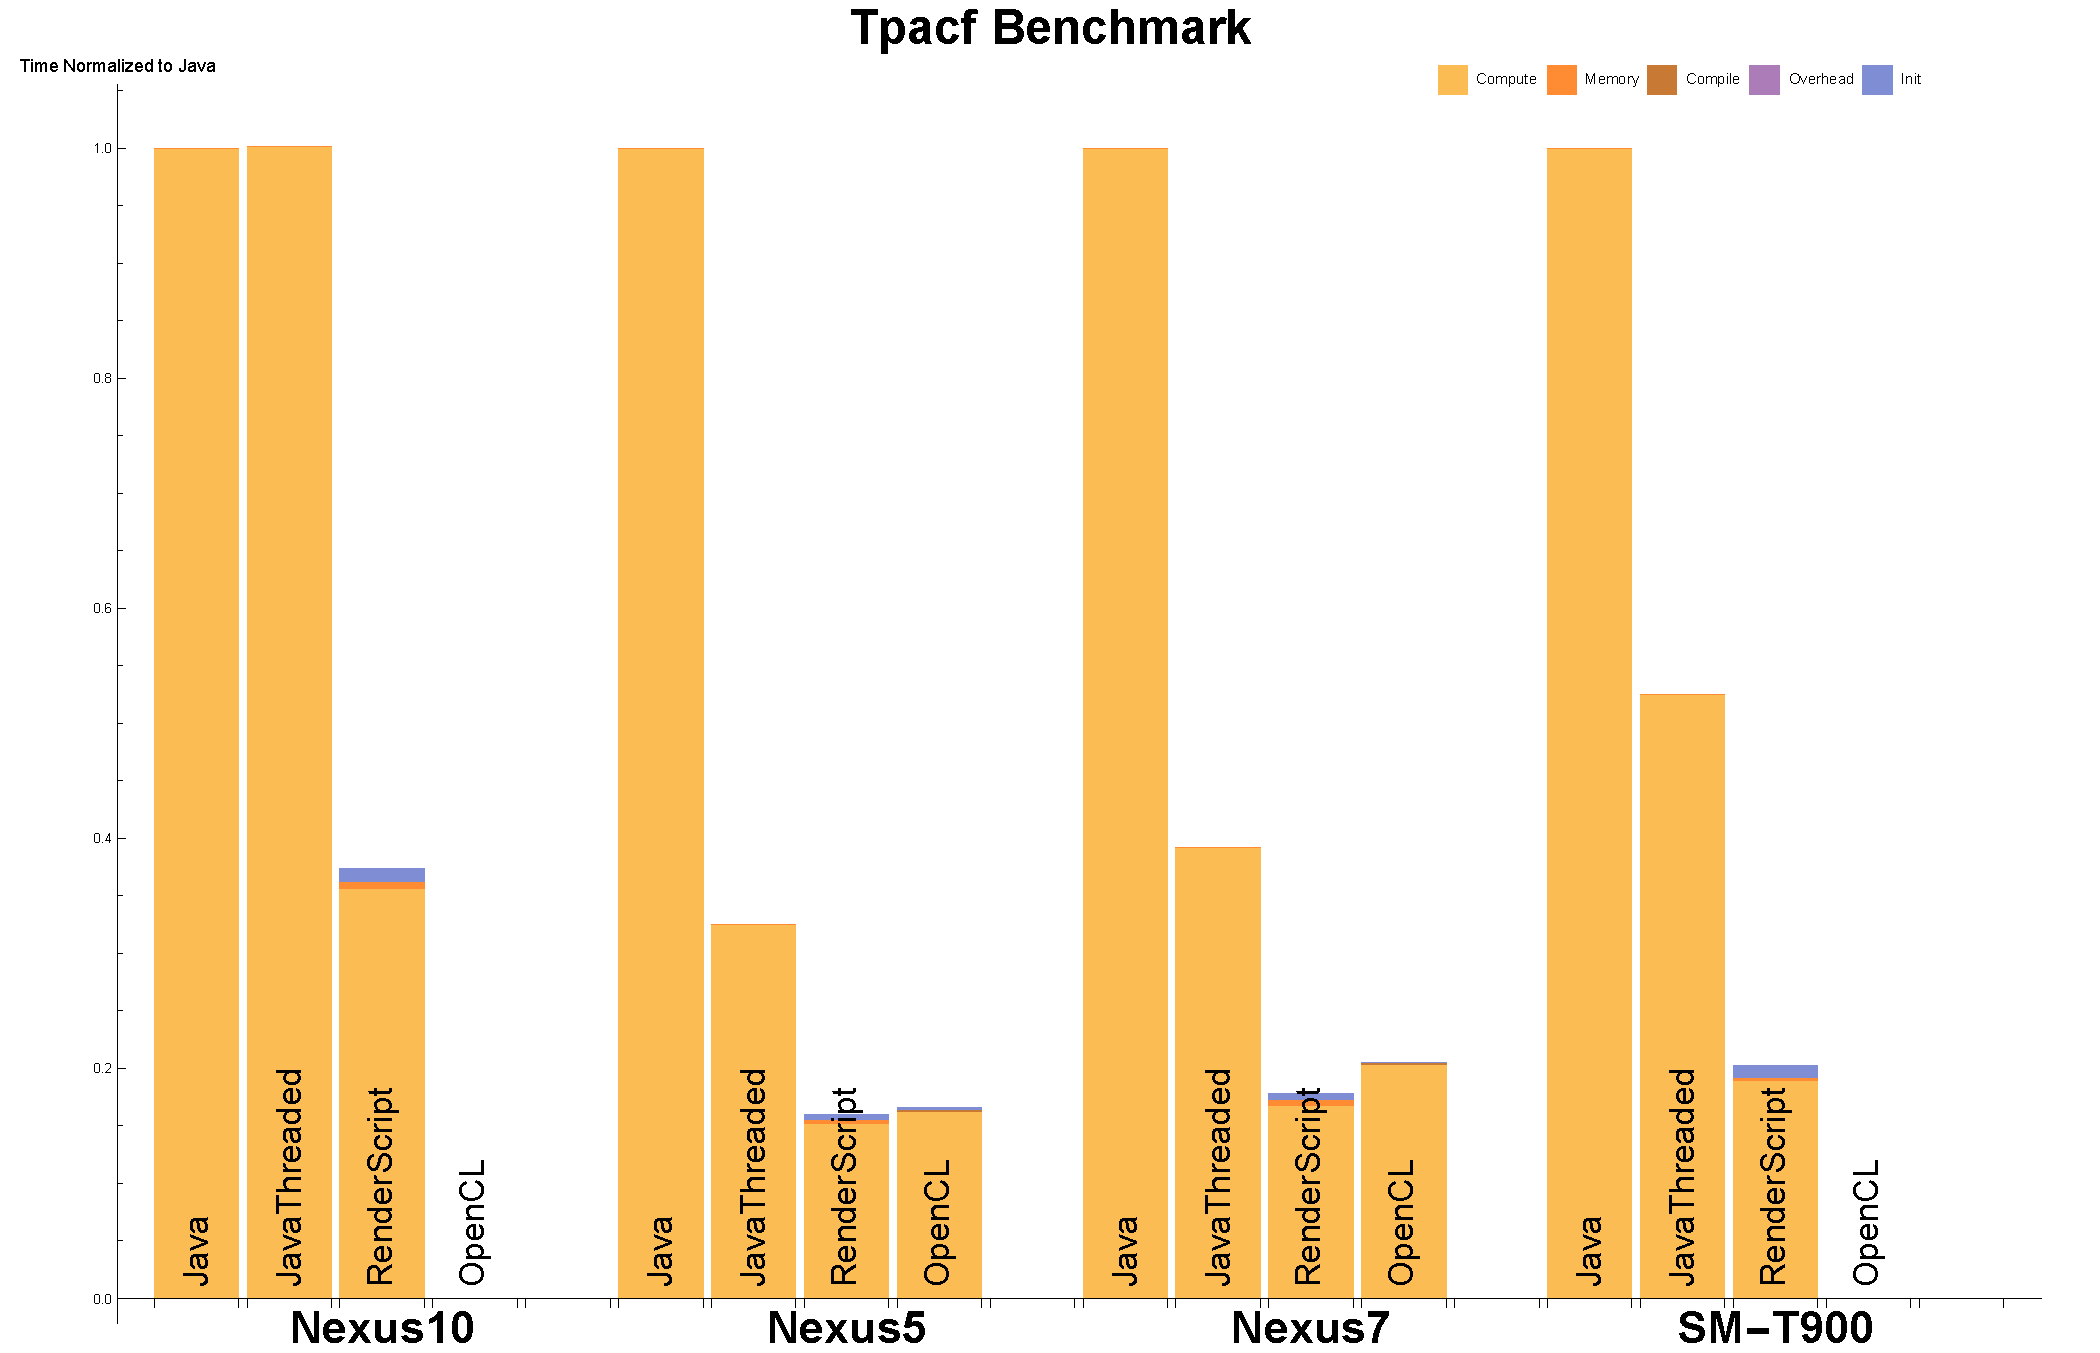
\includegraphics[width=0.9\textwidth]{data/Tpacf_time.pdf}
      \caption{TPACF}
  \end{subfigure}
  \begin{subfigure}[b]{0.33\textwidth}
      \centering
      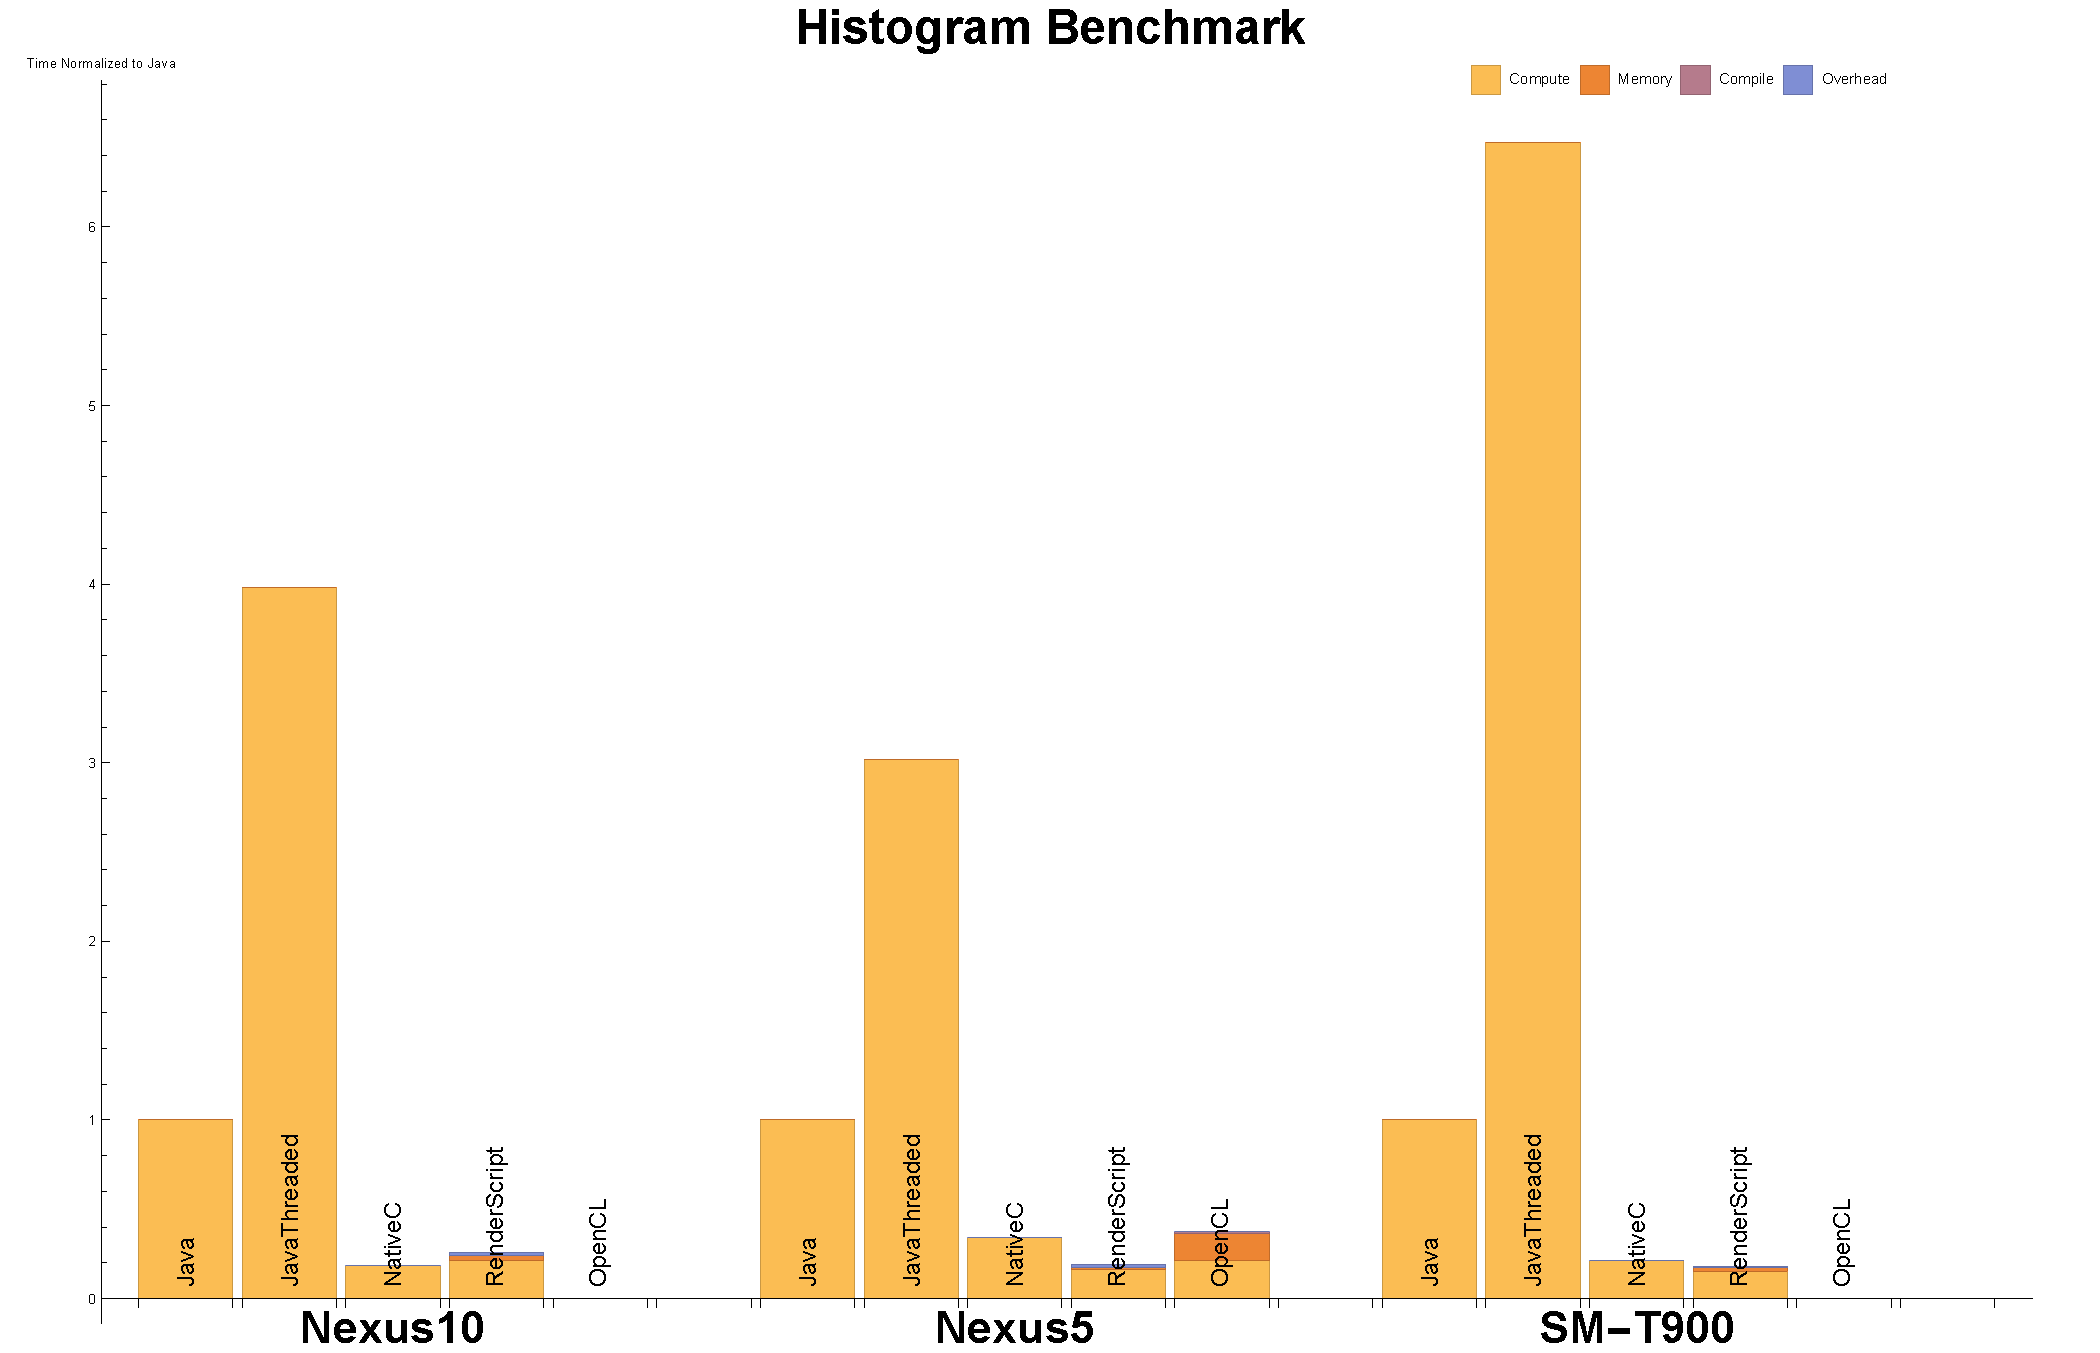
\includegraphics[width=0.9\textwidth]{data/Histogram_time.pdf}
      \caption{Histogram}
  \end{subfigure}
  \begin{subfigure}[b]{0.33\textwidth}
      \centering
      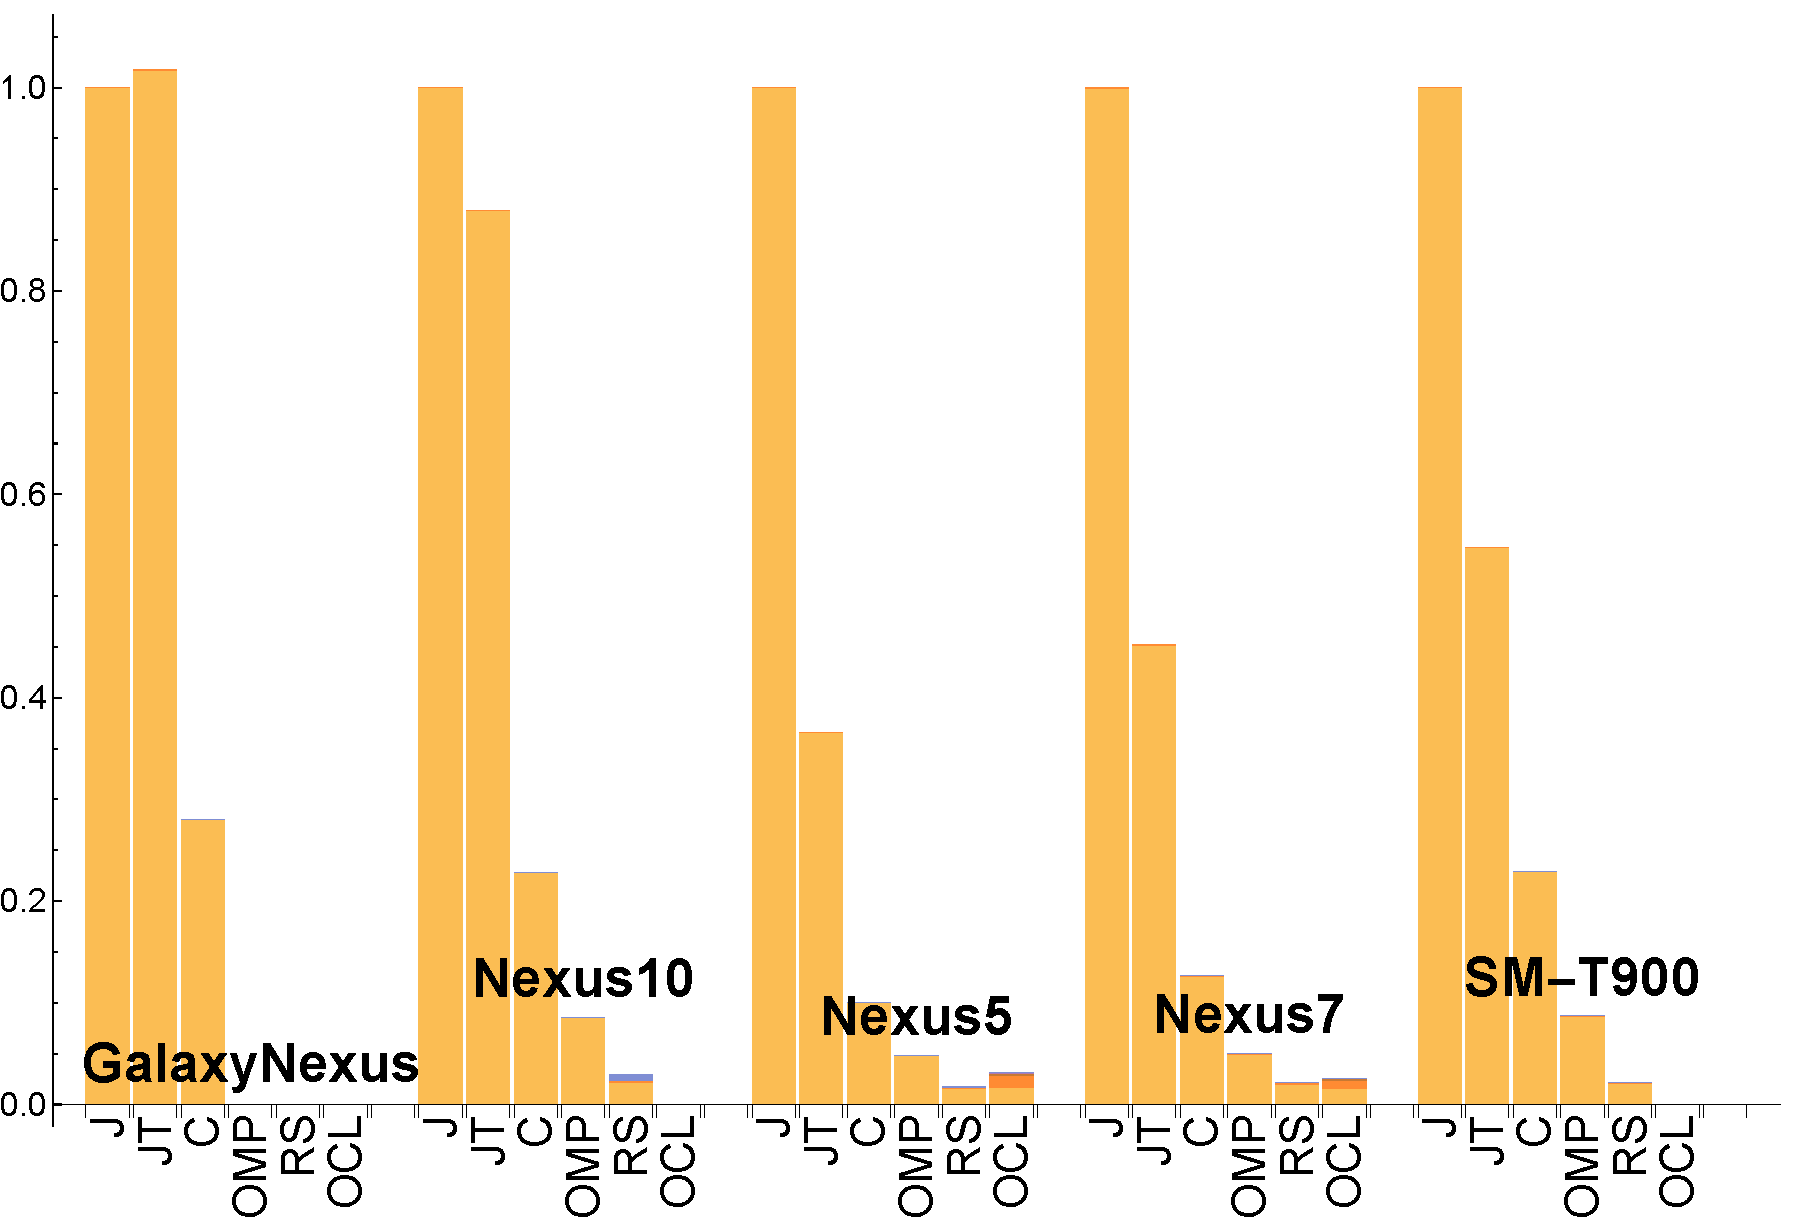
\includegraphics[width=0.9\textwidth]{data/Stencil_time.pdf}
      \caption{Stencil}
  \end{subfigure}

  \caption{Runtime across devices where kernel is executed multiple times. The runtimes are normalized to the Java execution time (lower is better). J : Java, JT : JavaThreaded, C : Native C, OMP: OpenMP, OCL : OpenCL, and RS : Renderscript.}
  \label{fig:perfMany}
\end{figure*}


The performance measurements are collected by measuring the time
  spent within each section of the code while the device is plugged
  into the development machine.
Each compute part of an implementation is run $5$ times with the minimum
  presented.
We consider two cases --- one where the kernel code is run once (figure~\ref{fig:perfOne}) and therefore
  the overhead (memory, compilation, and initialization) have an impact,
  and one where the kernel is run $100$ times (figure~\ref{fig:perfMany}) (or $5$ for both TPACF and MRIQ)
  and the overhead has little impact.

For each device, the plot show the time to execute sections of the code normalized
  to the Java execution time.
These times correspond to the $x$-axis of the processor utilization times discussed
  in the previous section (e.g. figure~\ref{fig:loadVecAddSgemm}) --- Trepn is not
  running while collecting these timing results.
Not all benchmarks were run on the GalaxyNexus, this is due to the device
  being low end resulting in a long time to execute some of the benchmarks.

In figure~\ref{fig:perfOne} the compute code is only executed once, it is clear that 
  the overhead of RenderScript on the Nexus 10 (and to some extent the SM-T900) device is consistentently high.
We suspect that the Nexus 5 and Nexus 7 are using a more recent version of the RenderScript library compared to the Nexus 10.
As one would expect, a kernel is executed only once is not a good fit to be ofloaded to either RenderScript or OpenCL.
This is due to overhead playing a big roll with overhead time being order of magnitude bigger than the compute time ---
  i.e. the programmer still needs to understand which sections of the program are very hot and could benifit by not being hosted 
  in Java.

In figure~\ref{fig:perfMany}, we look at the performance if memory management is optimized and the kernel code is executed 
  many times.
Code with a high memory to compute ratio, such as VectorAdd (and SGEMM to some extent), do not perform well using either
  RenderScript or OpenCL (this is due to poor occupancy in the OpenCL case).
For code that has irregular accesses or with a low memory to compute ratio, we see RenderScript's compute time to be similar
  to OpenCL, but is better when also considering overhead time.
Both RenderScript and OpenCL outperform the OpenMP implementation in all benchmarks as well.

As expected, the SGEMM OpenMP timing is similar to that of C, confirming our hypothesis that the compiler was not able
  to interpret the OpenMP pragma.
Because of the privatization, which requires an allocation in a thread, the threaded Java implementation performs poorly and is 
  worse than the serial Java implementation.
Consistently, OpenCL results in better speedups on the Nexus 5 versus the Nexus 7 when compared to the onboard CPU. 

The biggest performance gain comes by not using the JVM, however.
Aside from typical JVM overhead, we notice that these kernels are array access extensive.
Since Java's semantics garantee array accesses are within bounds, an overhead is encured.
Java's floating point semantics also do not match modern hardware (which implement the IEE 754 standard),
  this introduces more overhead where the JVM needs to perform extra checks.
These overheads do not manifest themselves in our native implementations.
We also use unsafe casts to reduce the overhead in the native implementations.

